% Editable native annotations around unchanged verified IDE photographs.
\par
\begin{figure}[htbp]
  \centering
  \sbox0{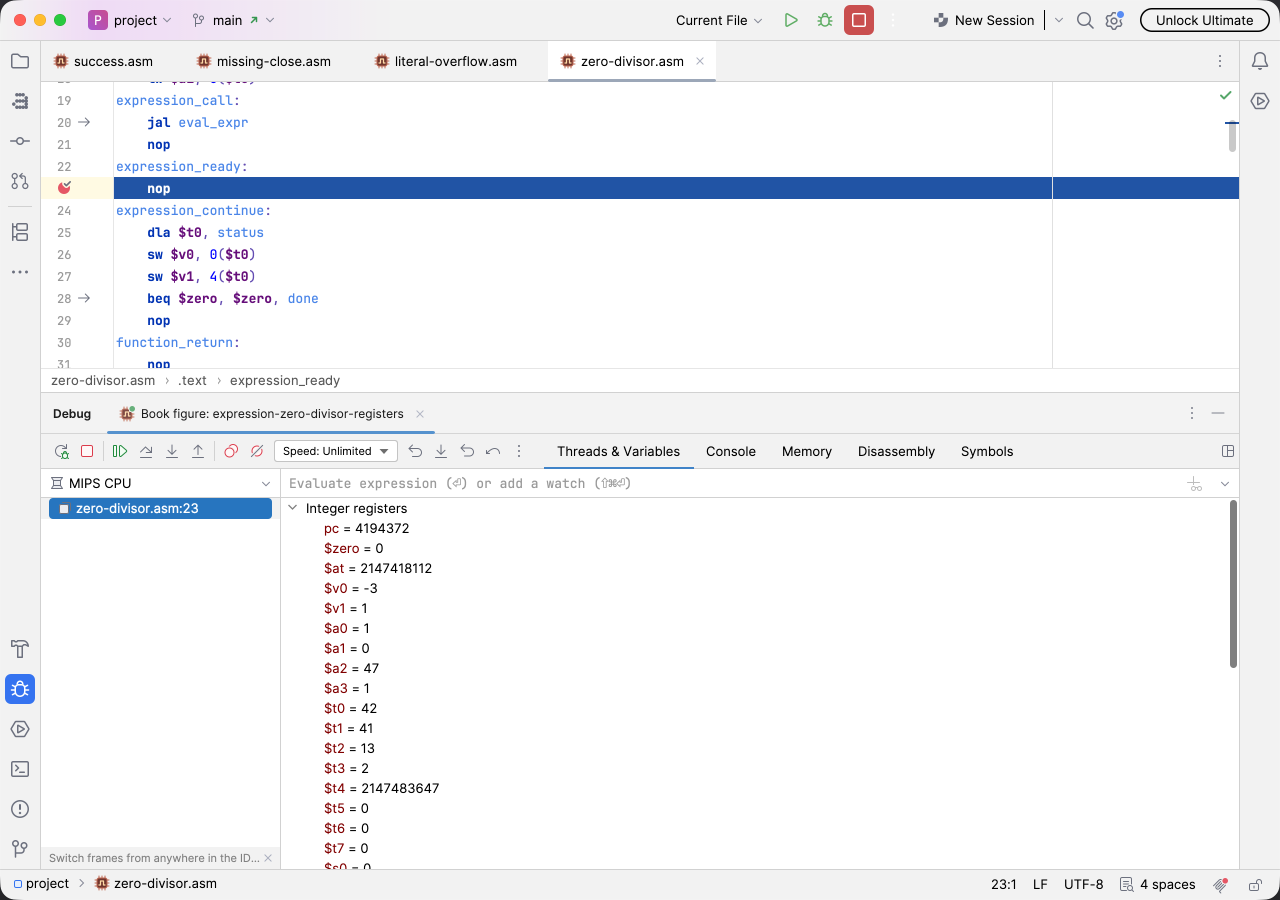
\includegraphics[artifact]{packages/017-expression-evaluator/captures/f04/registers.png}}
  \sbox2{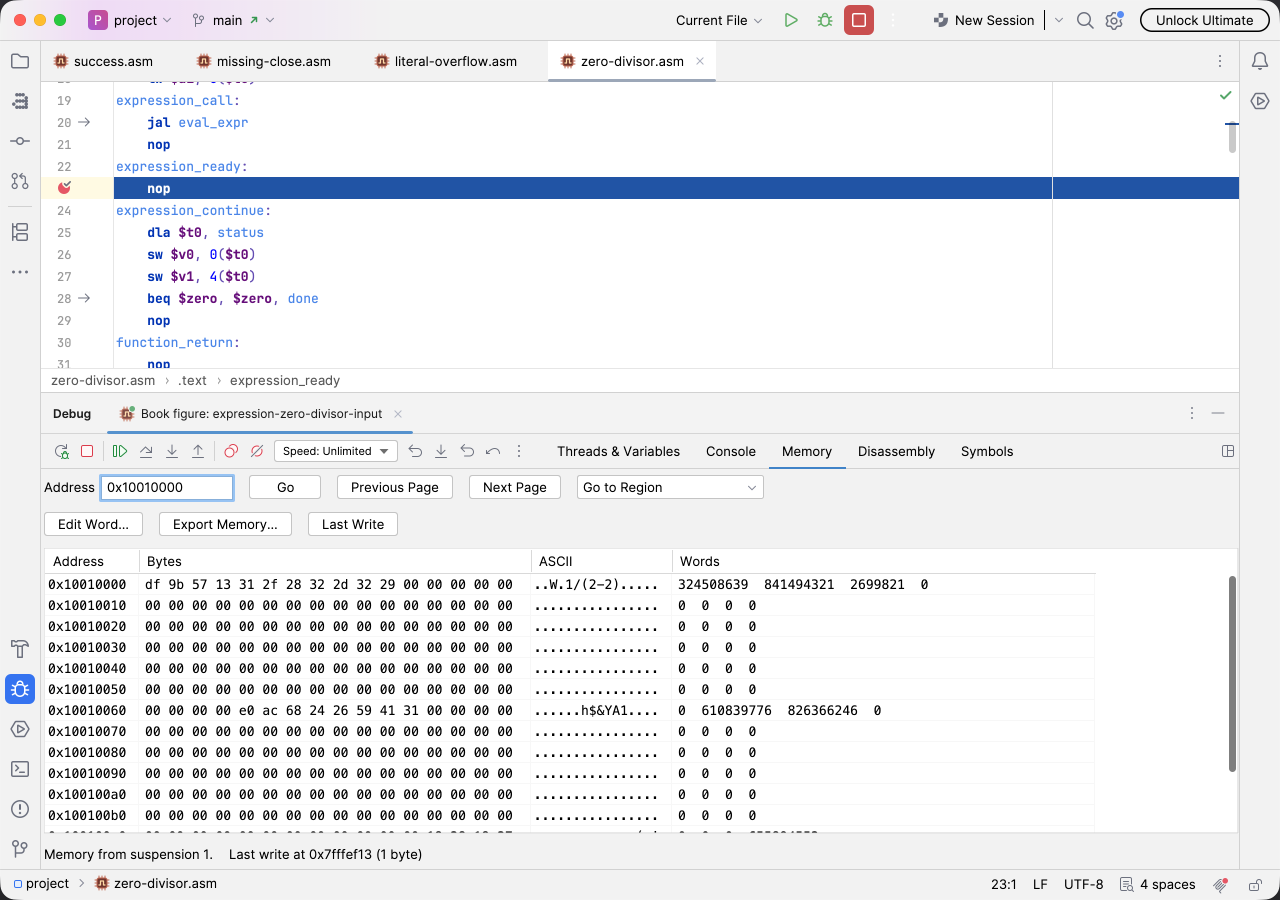
\includegraphics[artifact]{packages/017-expression-evaluator/captures/f04/input.png}}
  \sbox4{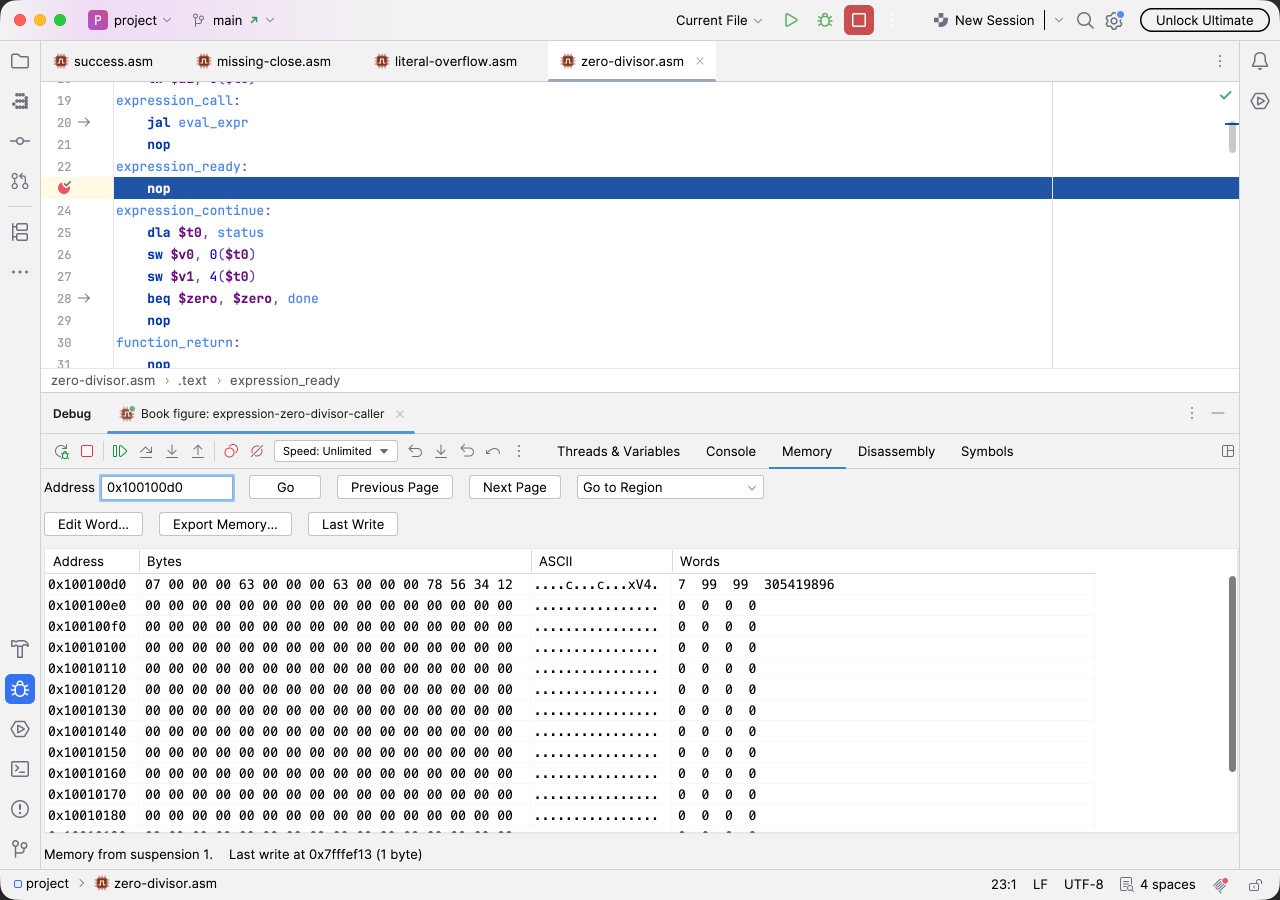
\includegraphics[artifact]{packages/017-expression-evaluator/captures/f04/caller.png}}
  \edef\MARSexpressionzerodivisorsourceLeft{\the\dimexpr0.036718750\wd0\relax}
  \edef\MARSexpressionzerodivisorsourceBottom{\the\dimexpr0.774444444\ht0\relax}
  \edef\MARSexpressionzerodivisorsourceRight{\the\dimexpr0.713281250\wd0\relax}
  \edef\MARSexpressionzerodivisorsourceTop{\the\dimexpr0.147777778\ht0\relax}
  \edef\MARSexpressionzerodivisorregistersLeft{\the\dimexpr0.246093750\wd0\relax}
  \edef\MARSexpressionzerodivisorregistersBottom{\the\dimexpr0.312222222\ht0\relax}
  \edef\MARSexpressionzerodivisorregistersRight{\the\dimexpr0.553906250\wd0\relax}
  \edef\MARSexpressionzerodivisorregistersTop{\the\dimexpr0.640000000\ht0\relax}
  \edef\MARSexpressionzerodivisorinputLeft{\the\dimexpr0.034375000\wd2\relax}
  \edef\MARSexpressionzerodivisorinputBottom{\the\dimexpr0.311111111\ht2\relax}
  \edef\MARSexpressionzerodivisorinputRight{\the\dimexpr0.584375000\wd2\relax}
  \edef\MARSexpressionzerodivisorinputTop{\the\dimexpr0.608888889\ht2\relax}
  \edef\MARSexpressionzerodivisorcallerLeft{\the\dimexpr0.034375000\wd4\relax}
  \edef\MARSexpressionzerodivisorcallerBottom{\the\dimexpr0.334444444\ht4\relax}
  \edef\MARSexpressionzerodivisorcallerRight{\the\dimexpr0.584375000\wd4\relax}
  \edef\MARSexpressionzerodivisorcallerTop{\the\dimexpr0.608888889\ht4\relax}
  \begin{tikzpicture}[alt={Four annotated details for the seven-byte input 1/(2-2). Native status is minus three and error offset one. The group closes successfully and supplies denominator zero. The slash at address 0x10010005 is the reported operator byte. The caller-memory row has length seven and both initial result words 99.}]
    \node[anchor=north west,inner sep=0,font=\small\bfseries] (source-title) at (6mm,0) {Next instruction after return};
    \node[anchor=north west,inner sep=0] (source) at ([yshift=-1mm]source-title.south west) {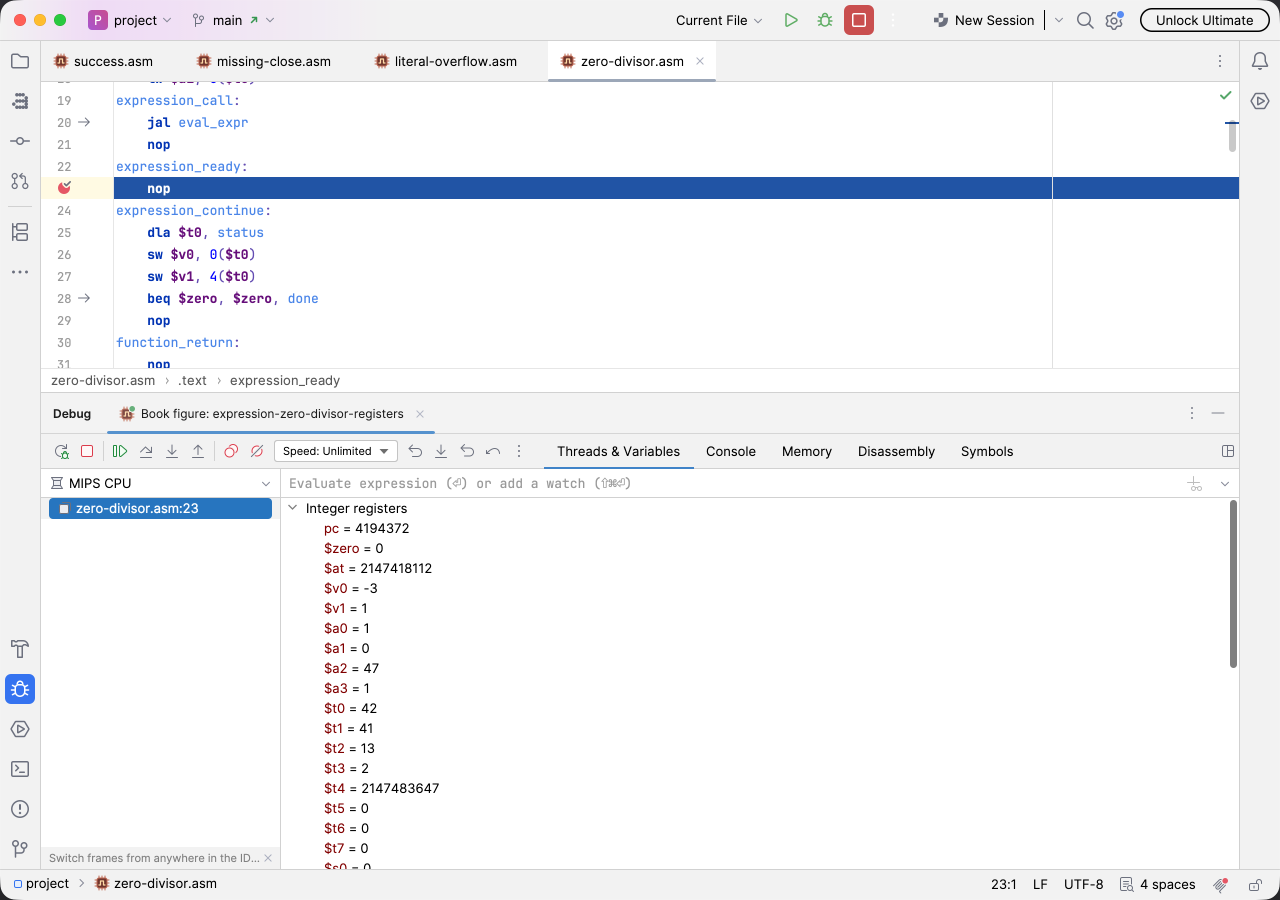
\includegraphics[width=0.54\linewidth,artifact,trim={\MARSexpressionzerodivisorsourceLeft{} \MARSexpressionzerodivisorsourceBottom{} \MARSexpressionzerodivisorsourceRight{} \MARSexpressionzerodivisorsourceTop{}},clip]{packages/017-expression-evaluator/captures/f04/registers.png}};
    \begin{scope}[shift={(source.south west)},x={($(source.south east)-(source.south west)$)},y={($(source.north west)-(source.south west)$)}]
      \draw[black,line width=0.7pt] (0.215625000,0.057142857) rectangle (0.384375000,0.371428571);
      \node[draw=black,fill=white,circle,inner sep=1.5pt,font=\footnotesize] at ($(0.215625000,0.371428571)+(-3mm,0)$) {1};
    \end{scope}
    \node[anchor=north west,inner sep=0,font=\small\bfseries] (registers-title) at (0.58\linewidth,0 |- source-title.north) {Signed return values};
    \node[anchor=north west,inner sep=0] (registers) at ([yshift=-1mm]registers-title.south west) {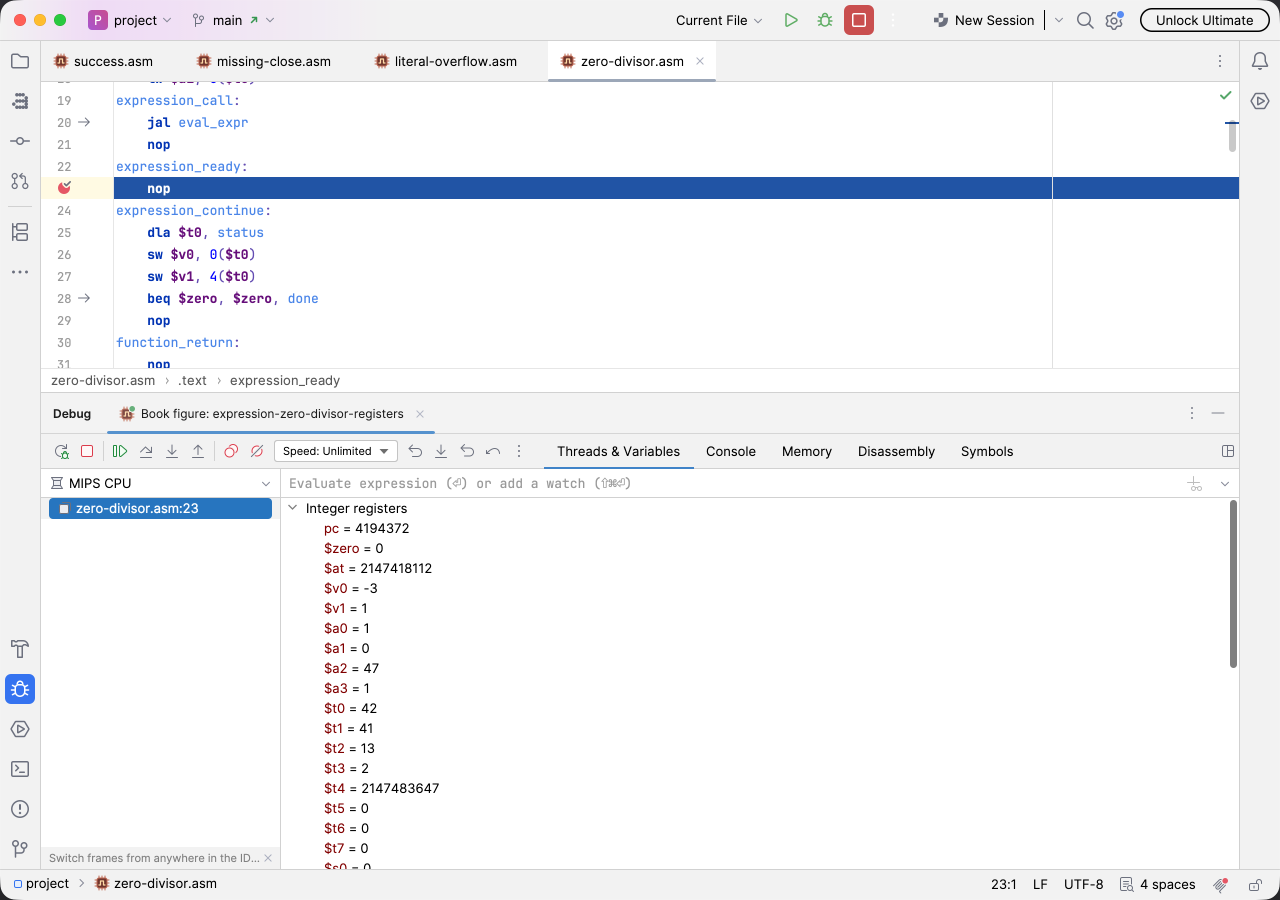
\includegraphics[width=0.42\linewidth,artifact,trim={\MARSexpressionzerodivisorregistersLeft{} \MARSexpressionzerodivisorregistersBottom{} \MARSexpressionzerodivisorregistersRight{} \MARSexpressionzerodivisorregistersTop{}},clip]{packages/017-expression-evaluator/captures/f04/registers.png}};
    \begin{scope}[shift={(registers.south west)},x={($(registers.south east)-(registers.south west)$)},y={($(registers.north west)-(registers.south west)$)}]
      \draw[black,line width=0.7pt] (0.023437500,0.023255814) rectangle (0.250000000,0.953488372);
      \node[draw=black,fill=white,circle,inner sep=1.5pt,font=\footnotesize] at ($(0.023437500,0.953488372)+(-3mm,0)$) {2};
    \end{scope}
    \node[anchor=north west,inner sep=0,font=\small\bfseries] (input-title) at ([yshift=-3mm]source.south west) {Input bytes, preceding guard and mapped padding};
    \node[anchor=north west,inner sep=0] (input) at ([yshift=-1mm]input-title.south west) {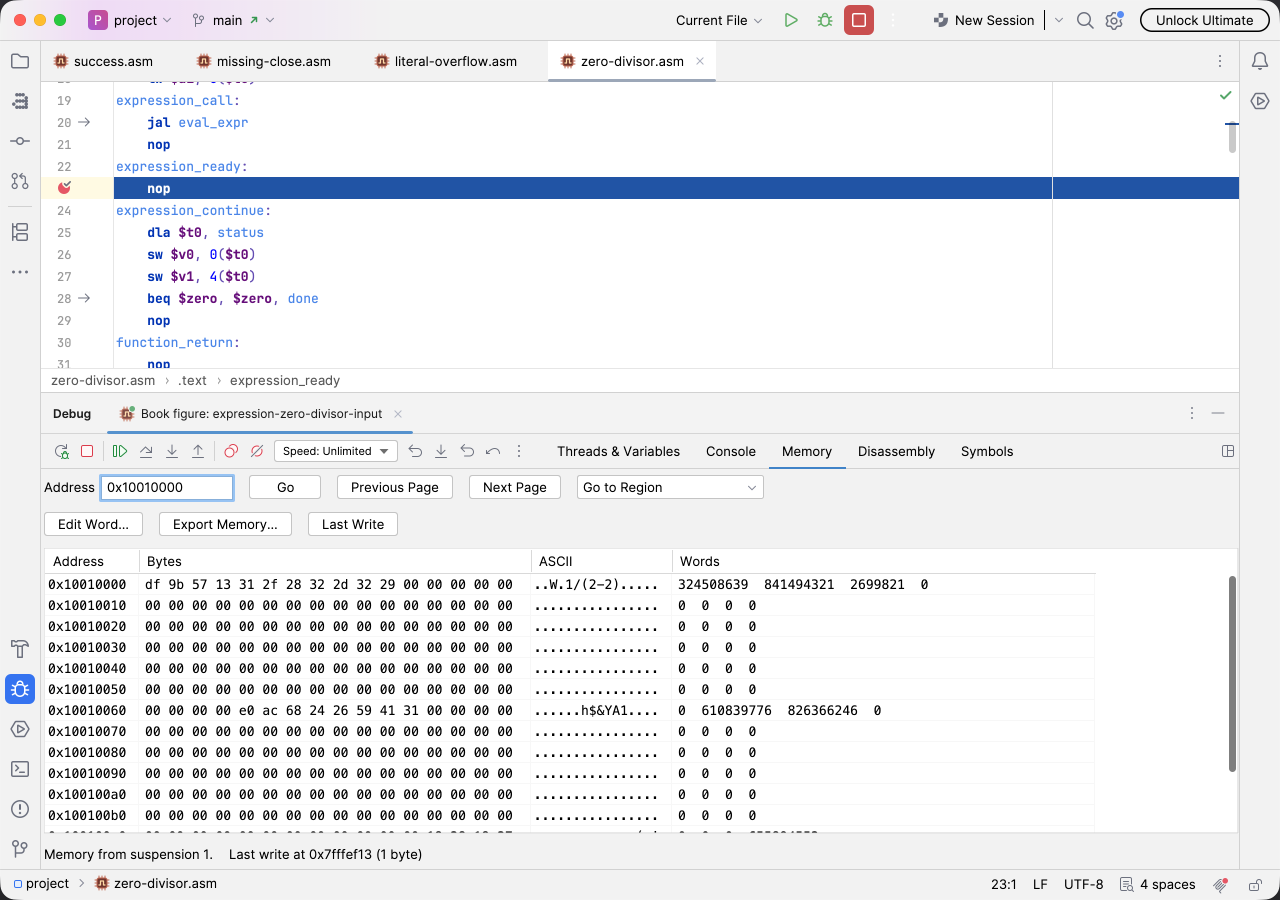
\includegraphics[width=0.84\linewidth,artifact,trim={\MARSexpressionzerodivisorinputLeft{} \MARSexpressionzerodivisorinputBottom{} \MARSexpressionzerodivisorinputRight{} \MARSexpressionzerodivisorinputTop{}},clip]{packages/017-expression-evaluator/captures/f04/input.png}};
    \begin{scope}[shift={(input.south west)},x={($(input.south east)-(input.south west)$)},y={($(input.north west)-(input.south west)$)}]
      \draw[black,line width=0.7pt] (0.194672131,0.055555556) rectangle (0.997950820,0.638888889);
      \node[draw=black,fill=white,circle,inner sep=1.5pt,font=\footnotesize] at ($(0,0.638888889)+(-3mm,0)$) {3};
    \end{scope}
    \node[anchor=north west,inner sep=0,font=\small\bfseries] (caller-title) at ([yshift=-3mm]input.south west) {Caller length and unpublished result words};
    \node[anchor=north west,inner sep=0] (caller) at ([yshift=-1mm]caller-title.south west) {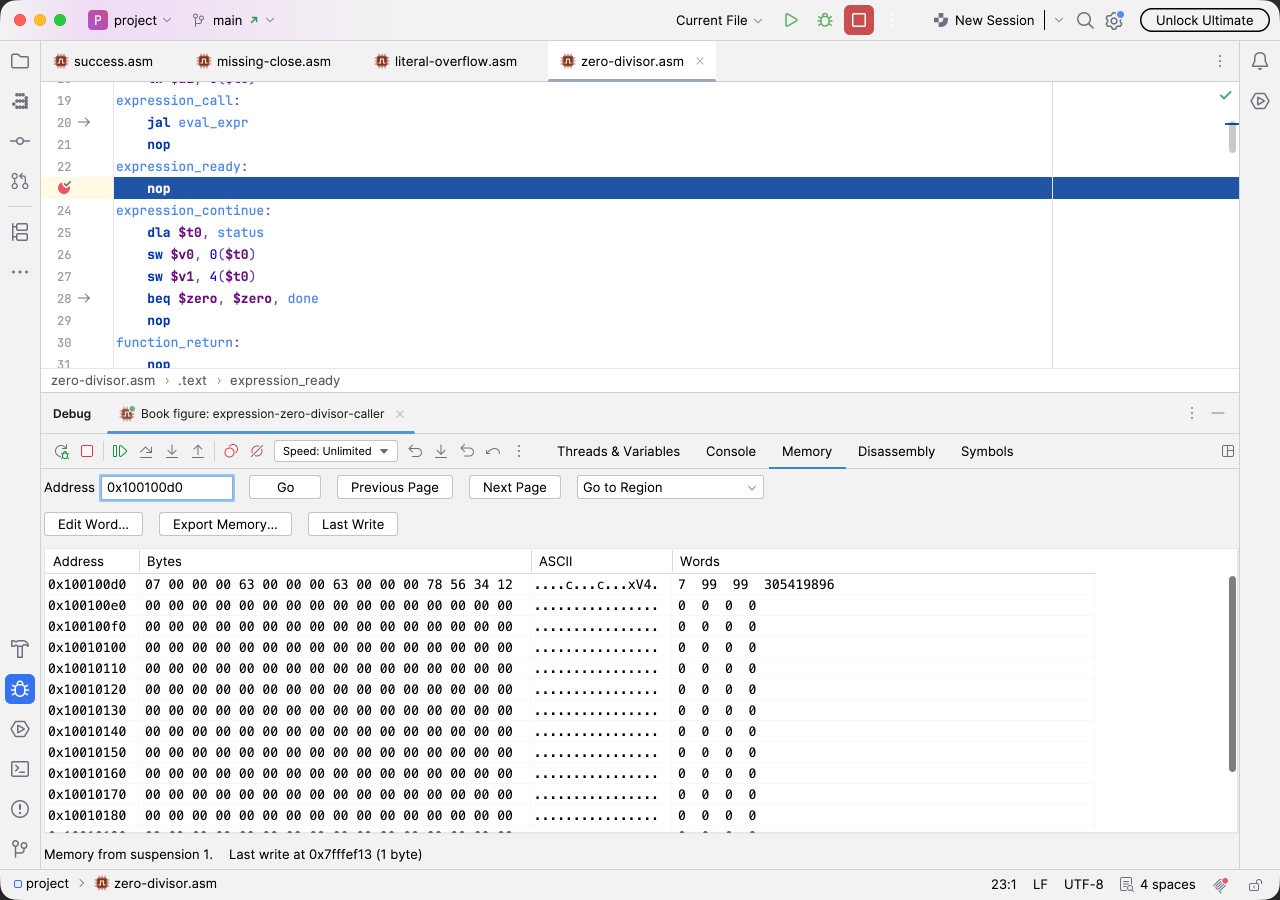
\includegraphics[width=0.84\linewidth,artifact,trim={\MARSexpressionzerodivisorcallerLeft{} \MARSexpressionzerodivisorcallerBottom{} \MARSexpressionzerodivisorcallerRight{} \MARSexpressionzerodivisorcallerTop{}},clip]{packages/017-expression-evaluator/captures/f04/caller.png}};
    \begin{scope}[shift={(caller.south west)},x={($(caller.south east)-(caller.south west)$)},y={($(caller.north west)-(caller.south west)$)}]
      \draw[black,line width=0.7pt] (0.194672131,0.078431373) rectangle (0.997950820,0.490196078);
      \node[draw=black,fill=white,circle,inner sep=1.5pt,font=\footnotesize] at ($(0,0.490196078)+(-3mm,0)$) {4};
    \end{scope}
  \end{tikzpicture}
  \par\smallskip
  \begin{minipage}{\linewidth}
    \small
    \begin{enumerate}
      \setlength{\itemsep}{2pt}
            \setlength{\parsep}{0pt}
      \item This fixture restores the closing parenthesis, supplying \texttt{1/(2-2)} with length 7. The complete group is now a valid right operand. Compare this return with the missing-close fixture; the one additional byte changes which failure the evaluator is allowed to report.
      \item \texttt{\$v0 = -3} reports division by zero. \texttt{\$v1 = 1} is the slash\textquotesingle s byte position. The grouped subtraction succeeds with value zero and its close is consumed before the binary operation checks that denominator. The error position names the failing operator, rather than the group\textquotesingle s last byte or the current cursor.
      \item The input starts at \texttt{0x10010004}; \texttt{2f} at the next address, \texttt{0x10010005}, is the slash at offset 1. The final \texttt{29} at offset 6 closes the group. All seven bytes are within the supplied slice, while the following zeros remain padding. Input and both surrounding allocations stay unchanged.
      \item The row at \texttt{0x100100d0} contains length, caller status, caller second result, and the final guard. Bytes \texttt{63 00 00 00} encode decimal 99, the initial value of both result words. The evaluator returns through registers and leaves caller data read-only. Continuing past \texttt{expression\_continue} lets the caller replace those two words; exit later reuses \texttt{\$v0} for its service number. Length is 7. The two stored 99 values are sentinels, not a successful expression result. After continuation, the caller stores status $-3$ and offset 1. Interpret that offset only together with its nonzero status.
    \end{enumerate}
  \end{minipage}
  \caption{A complete group returns zero, so division reports its operator at byte one.}
  \label{capture:017-expression-evaluator-f04}
  \label{expression-f04}
\end{figure}
\par
